% Act 1: the Mobileye fleet as the fan-out/fan-in picture; the map counts each road once (rule two).
\begin{frame}[t]{\ev{\tagO\,\tagP}A car fleet fans out, then fans in to one map.}
\vspace{.05cm}
\begin{columns}[T,onlytextwidth]
\column{.45\linewidth}
\vspace{.2cm}
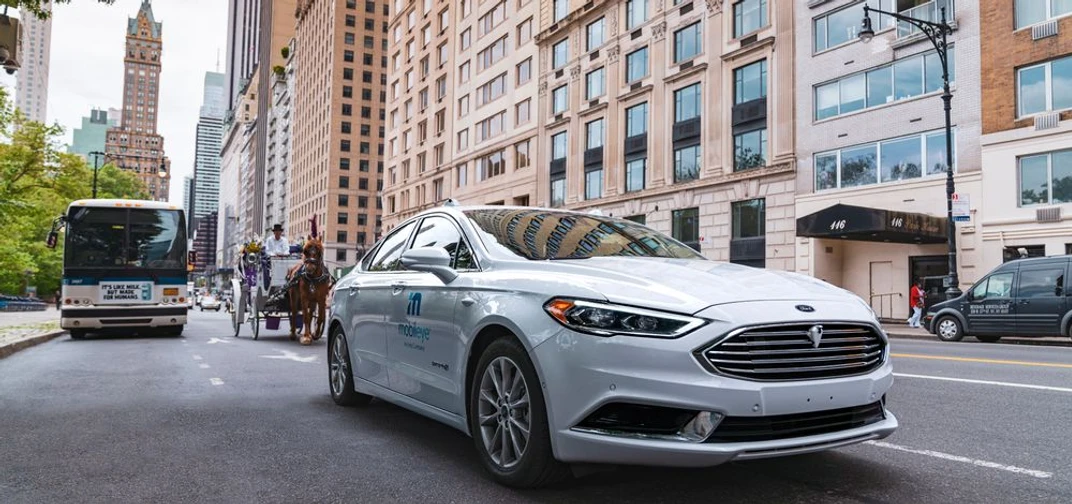
\includegraphics[width=\linewidth]{assets/mobileye-new-york-2021.png}\par
\tagline{Mobileye autonomous test vehicle,\\Manhattan, June 2021.}
\vspace{.12cm}
{\fontsize{11}{13}\selectfont\textbf{My work, 2021--2024:}\\junction perception.\par}
\column{.51\linewidth}
{\centering
\begin{tikzpicture}[x=1cm,y=1cm,every node/.style={align=center,font=\fontsize{11}{13}\selectfont}, side/.style={font=\fontsize{10}{11.5}\selectfont\bfseries,anchor=east}]
\node[font=\fontsize{11}{13}\selectfont\bfseries] at (0,3.25) {Assume 300 million cars send road data};
\foreach \k/\x in {1/-1.9,2/0,3/1.9}{\node[candidate,text width=1.25cm,minimum height=.6cm](c\k)at(\x,2.6){car};}
\node[evidence,text width=5.1cm,minimum height=.9cm](m)at(0,1.12){\textbf{Match the same road}\\combine repeated observations\\[3pt]{\setlength{\fboxsep}{1.7pt}\colorbox{Gold}{\textcolor{white}{\fontsize{7.6}{8.6}\selectfont\bfseries COUNT ONCE}}}};
\node[evidence,text width=5.1cm,minimum height=.9cm](r)at(0,-.5){\textbf{Roadbook map}\\sent back to cars};
\foreach \k in {1,2,3}{\draw[flow](c\k.south)--(m.north);}
\draw[flow](m)--(r);
\draw[message](r.east)--++(.35,0)|-(c3.east);
\node[side,text=Gold]at(-2.65,2.6){FAN\\OUT};
\node[side,text=Teal]at(-2.65,1.12){FAN\\IN};
\end{tikzpicture}\par}
\end{columns}
\claim{Self-driving compute: many runs from one state, one combined result.}
\sources{300M fleet: speaker-reported. \href{https://ir.mobileye.com/news-releases/news-release-details/mobileye-supply-cloud-enhanced-adas-select-future-stellantis}{Anonymized data flow}; \href{https://www.mobileye.com/technology/rem/}{Roadbook workflow}. Photo: \href{https://www.mobileye.com/press-kit/press-kit-mobileye-new-york-city/}{Mobileye press kit}.}
\qadetail{Fleet wording follows the speaker's request of 4 October 2026: assume 300 million Mobileye-equipped cars sensing roads and transmitting anonymized road data. The figure is supplied by the speaker from firsthand Mobileye experience and remains visibly attributed; it is not an independently verified public contributor count. The official 21 July 2026 release supports anonymized road-feature transmission to the cloud, processing and feedback to vehicles. That release reports a different, narrower mapping population: over eight million contributing vehicles and 34 billion road-miles in 2025 (about 1,080 road-miles per second as an annual average), alongside over 230 million vehicles built with EyeQ through 2025. These populations and dates do not establish a measured rate for the assumed 300-million-car fleet; no per-car transmission rate is asserted. The Roadbook workflow aligns repeated observations from the same road before combining them into a high-definition map of lanes, signs and driving paths and returning updates to cars. The COUNT ONCE chip is the talk's reading of that alignment step (many drives of one road are not independent roads), not a claim about Mobileye's statistical model. Parallel collection and aggregation motivate the computational fan-out/fan-in analogy without treating cars as checkpoint clones or repeated observations as independent evidence. The pictured vehicle is an autonomous test vehicle from Mobileye's Manhattan fleet, June 2021, as identified by the official press kit; it is not attributed to the speaker's team. The speaker's Mobileye employment, December 2021--March 2024, covered deep learning for production perception and road-junction semantics; personal junction-perception work is not authorship of the fleet mapping system. No Mobileye production accuracy or safety metric is asserted. The photo is the official image converted losslessly to PNG and scaled proportionally.}
\note{[0:45] Mobileye's Roadbook is a fleet example. Assume three hundred million equipped cars sending anonymized road observations. The cloud matches drives on the same road, combines them, and sends the updated map back to the cars. My own work there was junction perception. Notice that the map counts each road once, however many cars drove it. That is rule two. Self-driving compute gives execution the same shape: many runs from one reached state, one combined result.}
\end{frame}
